
\chapter{Comparison with experimental data}
\label{chap-experimental}

In order to validate the results produced by the software, several
test flights were made and compared to the results simulated by the
software.  In addition to the software produced, the same simulations
were performed in the current {\it de facto} standard model rocket simulator
RockSim~\cite{rocksim}.  The software used was the free demonstration
version of RockSim version 8.0.1f9.  This is the latest demo version
of the software available at the time of writing.  The RockSim site
states that the demo version is totally equivalent to the normal
version except that it can only be used a limited time and it does not
simulate the rocket's descent after apogee.

Comparisons were performed using both a typical model rocket design,
presented in Section~\ref{sec-comparison-small}, and a large hybrid
rocket, Section~\ref{sec-comparison-large}.  A small model with
canted fins was also constructed and flown to test the roll
simulation, presented in Section~\ref{sec-comparison-roll}.  Finally
in Section~\ref{sec-comparison-windtunnel} some of the the aerodynamic
properties calculated by the software are compared to actual
measurements performed in a wind tunnel.




\section{Comparison with a small model rocket}
\label{sec-comparison-small}

For purposes of gathering experimental flight data, a small model
rocket representing the size and characteristics of a typical model
rocket was constructed and flown in various configurations.  The
rocket model was 56~cm long with a body diameter of 29~mm.  The nose
cone was a 10~cm long tangent ogive, and the fins simple trapezoidal
fins.  The entire rocket was painted using an airbrush but not
finished otherwise and the fin profiles were left rectangular, so as
to represent a typical non-competition model rocket.  The velocity of
the rocket remained below 0.2~Mach during the entire flight.

In the payload section of the rocket was included an Alt15K/WD Rev2
altimeter from PerfectFlite~\cite{perfectflite}.  The altimeter
measures the altitude of the rocket based on atmospheric pressure
changes ten times per second. The manufacturer states the accuracy of
the altimeter to be $\pm (0.25\% + \rm 0.6~m)$.  The altimeter logs
the flight data, which can later be retrieved to a computer for
further analysis. 

Four holes, each 1~mm in diameter were drilled evenly around the
payload body to allow the ambient air pressure to reach the pressure
sensor, as per the manufacturer's instructions.  The rocket was
launched from a 1~m high tower launcher, which removed the need for
any launch lugs.  Figure~\ref{fig-rocket-picture} presents a
picture of the test rocket and the tower launcher.


\begin{figure}
\centering
\parbox{75mm}{\centering  % width 7.4cm
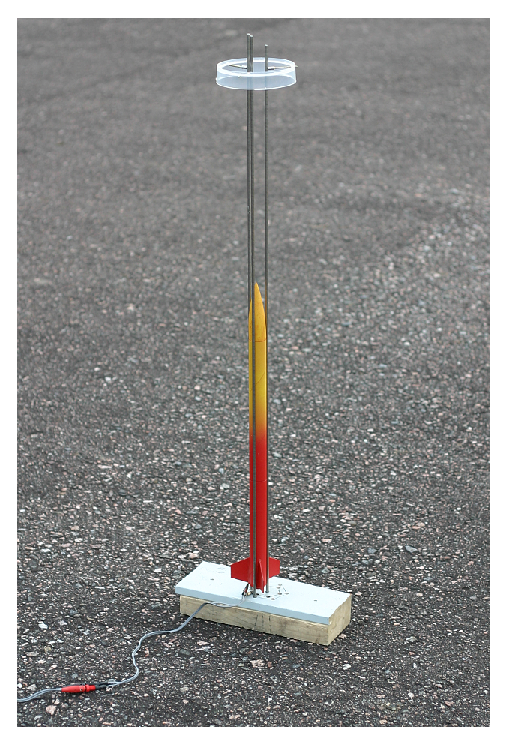
\epsfig{file=figures/pix/rocket-tower,height=11cm} \\ (a)}
\hspace{10mm}
\parbox{35mm}{\centering  % width 3.4cm
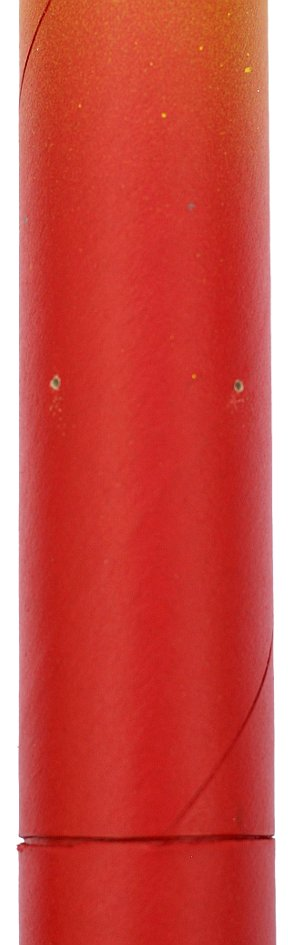
\epsfig{file=figures/pix/rocket-closeup,height=11cm} \\ (b)}
%
\caption{The test rocket awaiting launch on the tower launcher (a) and
  a close-up of its ventilation holes (b).}
\label{fig-rocket-picture}
\end{figure}


A design of the same rocket was created in both OpenRocket and
RockSim.  During construction of the rocket each component was
individually weighed and the weight of the corresponding component
was overridden in the software for maximum accuracy.  Finally, the 
mass and CG position of the entire rocket was overridden with measured
values.

One aspect of the rocket that could not be measured was the average
surface roughness.  In the OpenRocket design the ``regular paint''
finish was selected, which corresponds to an average surface roughness
of 60~\textmu m.  From the available options of ``polished'',
``gloss'', ``matt'' and ``unfinished'' in RockSim, the ``matt'' option
was estimated to best describe the rocket; the corresponding
average surface roughness is unknown.

The rocket was flown using motors manufactured by WECO Feuerwerk
(previously Sachsen Feuerwerk)~\cite{weco-feuerwerk}, which correspond
largely to the motors produced by Estes~\cite{estes}.  The only source
available for the thrust curves of Sachsen Feuerwerk motors was a
German rocketry store~\cite{sf-thrustcurves}, the original source of
the measurements are unknown.  The thrust curve for the C6-3 motor is
quite similar to the corresponding Estes motor, and has a total impulse
of 7.5~Ns.  However, the thrust curve for the B4-4 motor yields a
total impulse of 5.3~Ns, which would make it a C-class motor, while
the corresponding Estes motor has an impulse of only 4.3~Ns.  Both
OpenRocket and RockSim simulated the flight of the rocket using the
SF B4-4 motor over 60\% higher than the apogee of the experimental
results.  It is likely that the thrust curve of the SF B4-4 is wrong,
and therefore the Estes B4-4 motor was used in the simulations in its
stead.


\begin{table}
\caption{Apogee altitude of simulated and experimental flights with
  B4-4 and C6-3 motors.}
\label{tab-flight-results}
\begin{center}
\begin{tabular}{ccccc}
             & \multicolumn{2}{c}{B4-4} & \multicolumn{2}{c}{C6-3} \\
\hline
Experimental~~~~ & 64.0 m &       & 151.5 m &       \\
OpenRocket~~~~   & 74.4 m & +16\% & 161.4 m & +7\%  \\
RockSim~~~~      & 79.1 m & +24\% & 180.1 m & +19\% \\
\hline
\end{tabular}
\end{center}
\end{table}


Figure~\ref{fig-flight-B4} shows the experimental and simulated
results for the flight using a B4-4 motor (simulations using an Estes
motor) and figure~\ref{fig-flight-C6} using a C6-3 motor.  The RockSim
simulations are truncated at apogee due to limitations of the
demonstration version of the software.  A summary of the apogee
altitudes is presented in Table~\ref{tab-flight-results}.  

Both simulations produce a bit too optimistic results. OpenRocket
yielded altitudes 16\% and 7\% too high for the B4-4 and C6-3 motors,
respectively, while RockSim had errors of 24\% and 19\%.  The C6-3
flight is considered to be more accurate due to the ambiguity of the
B4-4 thrust curve.
%
Another feature that can be seen from the graphs is that the estimated
descent speed of the rocket is quite close to the actual descent
speed.  The error in the descent speeds are 7\% and 13\% respectively.


\begin{figure}[p]
\centering
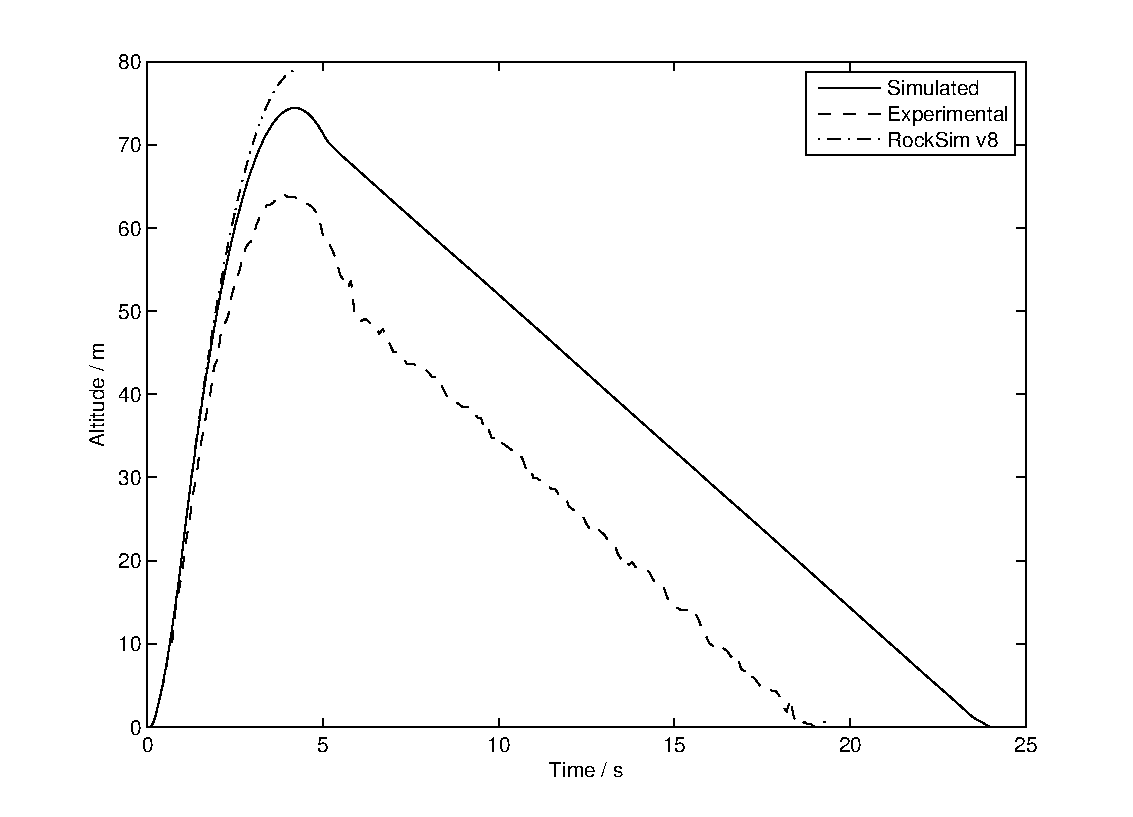
\epsfig{file=figures/experimental/flight-B4-4,width=12cm}
\caption{Experimental and simulated flight using a B4-4 motor.}
\label{fig-flight-B4}
\end{figure}

\begin{figure}[p]
\centering
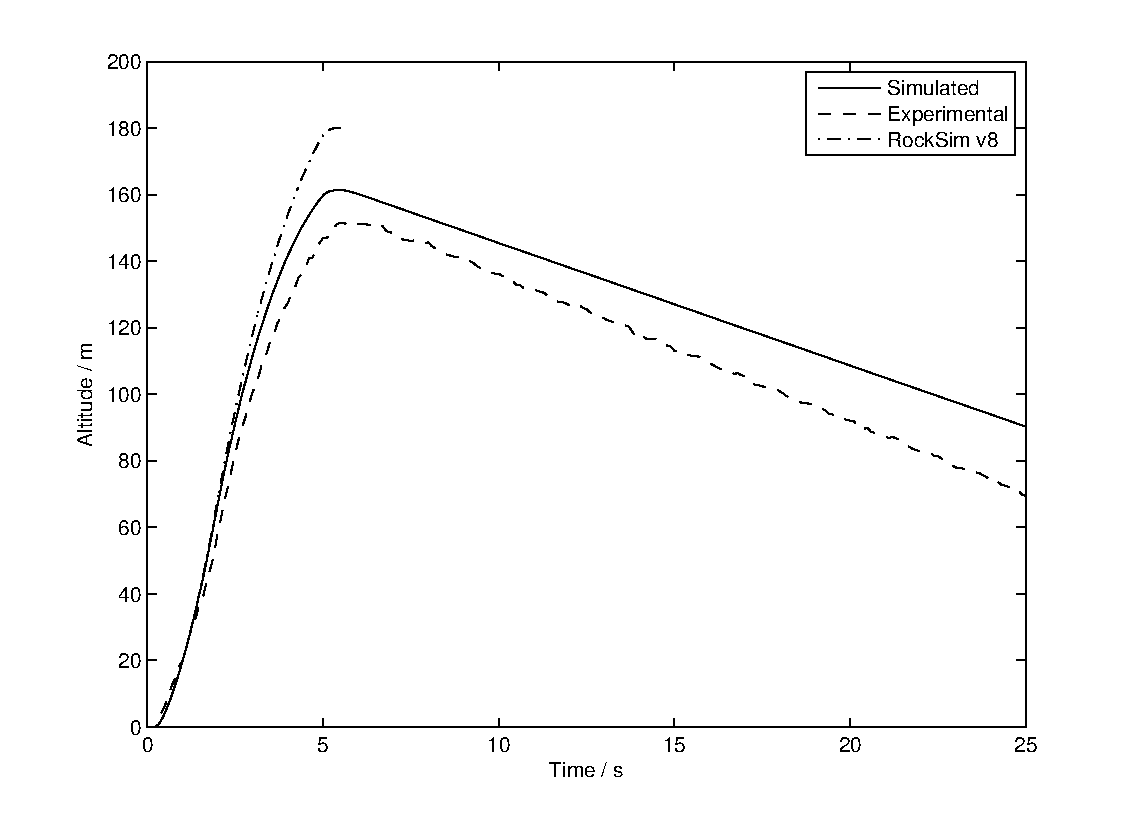
\epsfig{file=figures/experimental/flight-C6-3,width=12cm}
\caption{Experimental and simulated flight using a C6-3 motor.}
\label{fig-flight-C6}
\end{figure}


%       B4-4               C6-3
%Exp    64.0               151.5
%OR     74.4 +10.4 +16%    161.4 +9.9  +7%
%RS     79.1 +15.1 +24%    180.1 +28.6 +19%


The rocket was also launched with a launch lug 24~mm long and 5~mm in
diameter attached first to its mid-body and then next to its fins to
test the effect of a launch lug on the aerodynamic drag.  The apogee
altitudes of the tests were 147.2~m and 149.0~m, which correspond to
an altitude reduction of 2--3\%.  The OpenRocket simulation with such
a launch lug yielded results approximately 1.3\% less than without the
launch lug.




\section{Comparison with a hybrid rocket}
\label{sec-comparison-large}

The second comparison is with the Haisun��t� hybrid
rocket~\cite{haisunaata-launch}, which was launched in September 2008.
The rocket is a HyperLOC 835 model, with a length of 198~cm and a body
diameter of 10.2~cm.  The nose cone is a tangent ogive with a length
of 34~cm, and the kit includes three approximately trapezoidal fins.

The flight computer on board was a miniAlt/WD altimeter by
PerfectFlite~\cite{perfectflite}, with a stated accuracy of 
$\pm0.5\%$.  The flight computer calculates the altitude 20 times per
second based on the atmospheric pressure and stores the data into
memory for later analysis.

The rocket was modeled as accurately as possible with both OpenRocket
and RockSim, but the mass and CG of each component was computed by the
software.  Finally, the mass of the entire rocket excluding the motor
was overridden by the measured mass of the rocket.  The surface
roughness was estimated as the same as for the small rocket,
60~\textmu m in OpenRocket and ``matt'' for RockSim.

Figure~\ref{fig-flight-haisunaata} presents the true flight profile
and that of the simulations.  Both OpenRocket and RockSim estimate a
too low apogee altitude, with an error of 16\% and 12\%,
respectively.  As in the case of the small rocket model, RockSim
produces an estimate 5--10\% higher than OpenRocket.  It remains
unclear which software is more accurate in its estimates.

% Experimental 965m
% OpenRocket 814m
% RockSim  853m


One error factor also affecting this comparison is the use of a hybrid
rocket motor.  As noted in Section~\ref{sec-motors}, the vapor
pressure of the nitrous oxide is highly dependent on temperature,
which affects the thrust of the motor.  This may cause some variation
in the thrust between true flight and motor tests.

\begin{figure}[p]
\centering
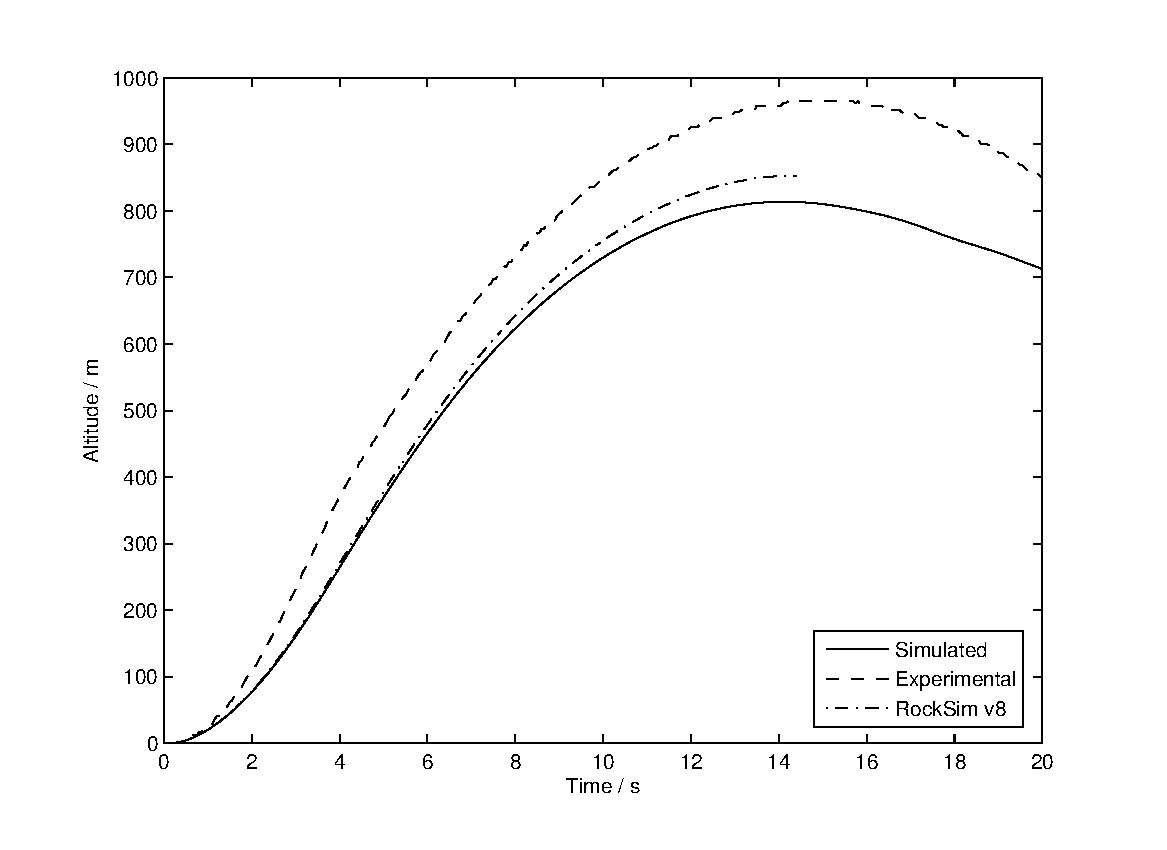
\epsfig{file=figures/experimental/flight-haisunaata,width=12cm}
\caption{Experimental and simulated flight of a hybrid rocket.}
\label{fig-flight-haisunaata}
\end{figure}

\begin{figure}[p]
\centering
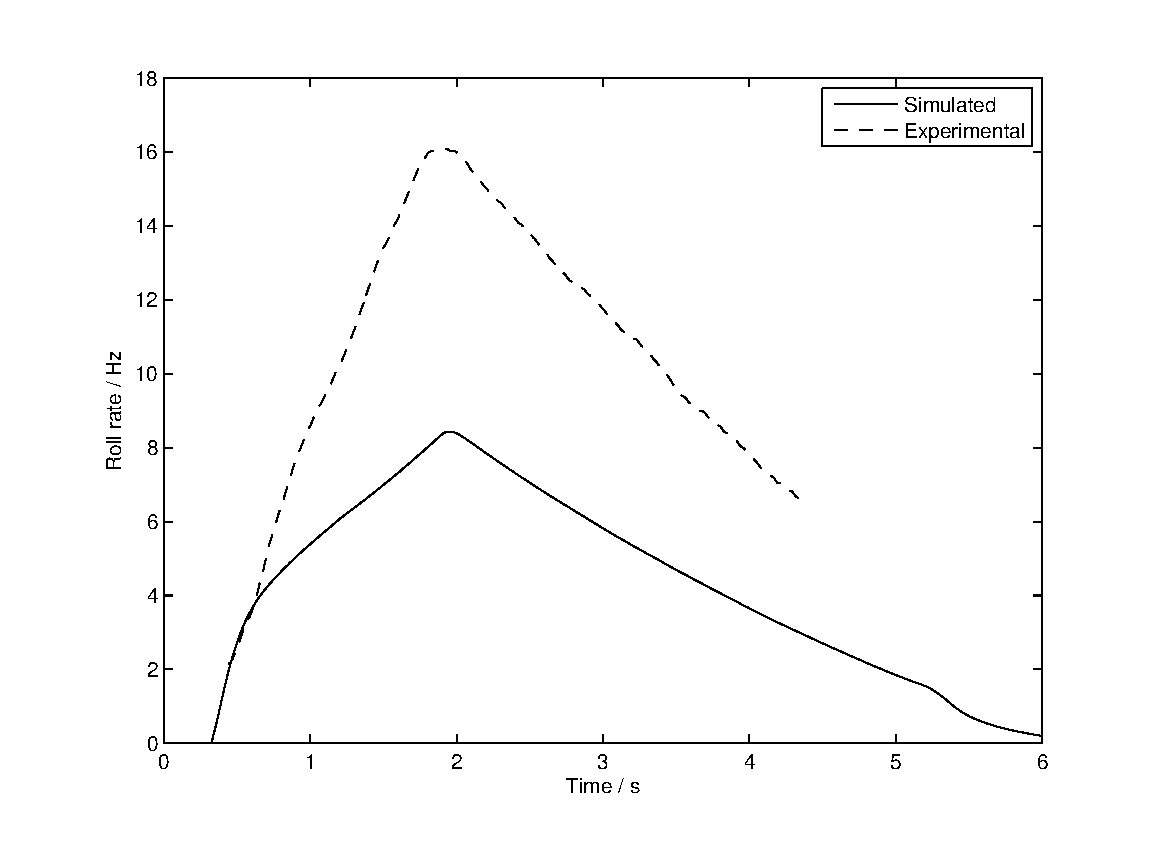
\epsfig{file=figures/experimental/flight-roll-rate,width=12cm}
\caption{Experimental and simulated roll rate results using a C6-3
  motor.}
\label{fig-flight-roll}
\end{figure}



\section{Comparison with a rolling rocket}
\label{sec-comparison-roll}

In order to test the rolling moment computation, a second
configuration of the small model rocket, described in
Section~\ref{sec-comparison-small}, was built with canted fins.  The
design was identical to the previous one, but each fin was canted by
an angle of $5^\circ$.  In addition, the payload section contained a
magnetometer logger, built by Antti~J. Niskanen, that measured the
roll rate of the rocket.  The logger used two Honeywell HMC1051
magnetometer sensors to measure the Earth's magnetic field and store
the values at a rate of 100~Hz for later analysis.  The rocket was
launched from the tower launcher using a Sachsen Feuerwerk C6-3
motor.  Further test flights were not possible since the lower rocket
part was destroyed by a catastrophic motor failure on the second
launch.

After the flight, a spectrogram of the magnetometer data was generated
by dividing the data into largely overlapping segments of 0.4~seconds each,
windowed by a Hamming window, and computing the Fourier transform of
these segments.  For each segment the frequency with the largest power
density was chosen as the roll frequency at the midpoint of the
segment in time.  The resulting roll frequency as a function of time
is plotted in Figure~\ref{fig-flight-roll} with the corresponding
simulated roll frequency.


The simulated roll rate differs significantly from the experimental
roll rate.  During the flight the rocket peaked at a roll rate of 16
revolutions per second, while the simulation has only about half of
this.  The reason for the discrepancy is unknown and would need more
data to analyze.  However, after the test flight it was noticed that
the cardboard fins of the test rocket were slightly curved, which may
have a significant effect on the roll rate.  A more precise test rocket
with more rigid and straight fins would be needed for a more
definitive comparison.  Still, even at a cant angle of $7^\circ$ the
simulation produces a roll rate of only 12~r/s.

Even so, it is believed that including roll in the simulation allows
users to realistically analyze the effect of roll stabilization for
example in windy conditions.


\section{Comparison with wind tunnel data}
\label{sec-comparison-windtunnel}


Finally, the simulated results were compared with experimental wind
tunnel data.  The model that was analyzed by J.~Ferris in the
transonic region~\cite{experimental-transonic} and by C.~Babb and
D.~Fuller in the supersonic region~\cite{experimental-supersonic} is
representative of the Arcas Robin meteorological rocket that has been
used in high-altitude research activities.  The model is 104.1~cm long
with a body diameter of 5.72~cm.  It includes a 27~cm long tangent
ogive nose cone and a 4.6~cm long conical boattail at the rear end,
which reduces the diameter to 3.7~cm.  The rocket includes four
trapezoidal fins, the profiles of which are double-wedges.  For
details of the configuration, refer to~\cite{experimental-transonic}.

The design was replicated in OpenRocket as closely as possible,
given the current limitations of the software.  The most notable
difference is that an airfoil profile was selected for the fins
instead of the double-wedge that is not supported by OpenRocket.  The
aerodynamical properties were computed at the same Mach and Reynolds
numbers as the experimental data.


\begin{figure}[t]
\centering
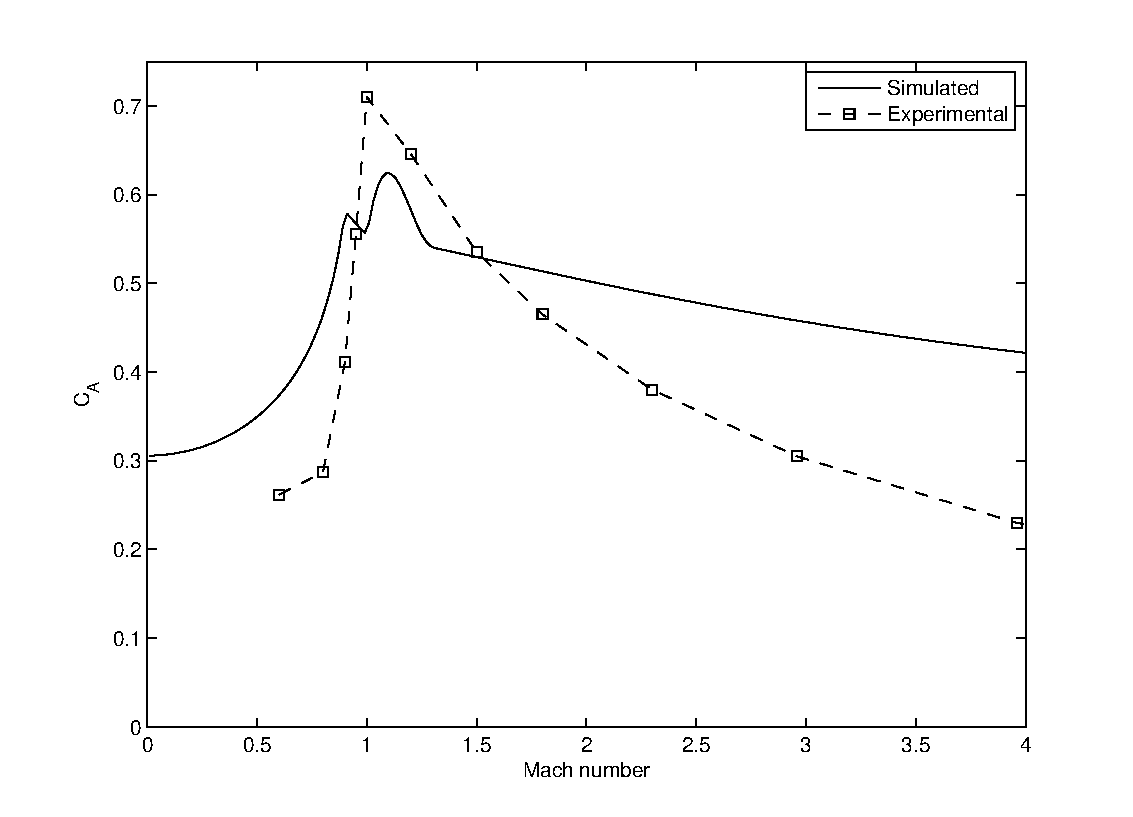
\epsfig{file=figures/experimental/ca-vs-mach,width=11cm}
\caption{Experimental and simulated axial drag coefficient as a
  function of Mach number.}
\label{fig-experimental-CA}
\end{figure}

The most important variables affecting the altitude reached by a
rocket are the drag coefficient and CP location.  The experimental and
simulated axial drag coefficient at zero angle-of-attack is presented
in Figure~\ref{fig-experimental-CA}.  The general shape of the
simulated drag coefficient follows the experimental results.  However,
a few aspects of the rocket break the assumptions made in the
computation methods.  First, the boattail at the end of the rocket
reduces the drag by guiding the air into the void left behind it,
while the simulation software only takes into account the reduction of
base area.  Second, the airfoil shape of the fins affects the drag
characteristic especially in the transonic region, where it produces
the slight reduction peak.  Finally, at higher supersonic speeds the
simulation produces less reliable results as expected, producing a too
high drag coefficient.  Overall, however, the drag coefficient matches
the experimental results with reasonable accuracy, and the results of
actual test flights shown in Sections~\ref{sec-comparison-small} and
\ref{sec-comparison-large} give credence to the drag coefficient
estimation.


\begin{figure}
\centering
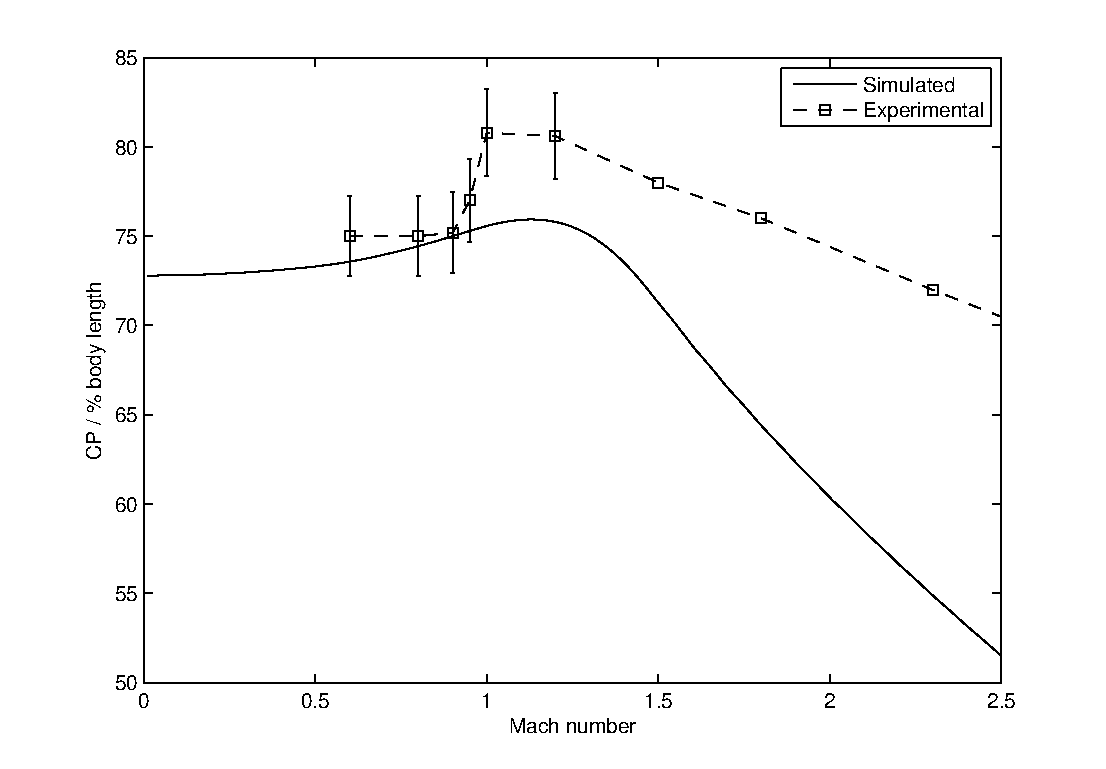
\epsfig{file=figures/experimental/cp-vs-mach,width=12cm} \\
(a) \\
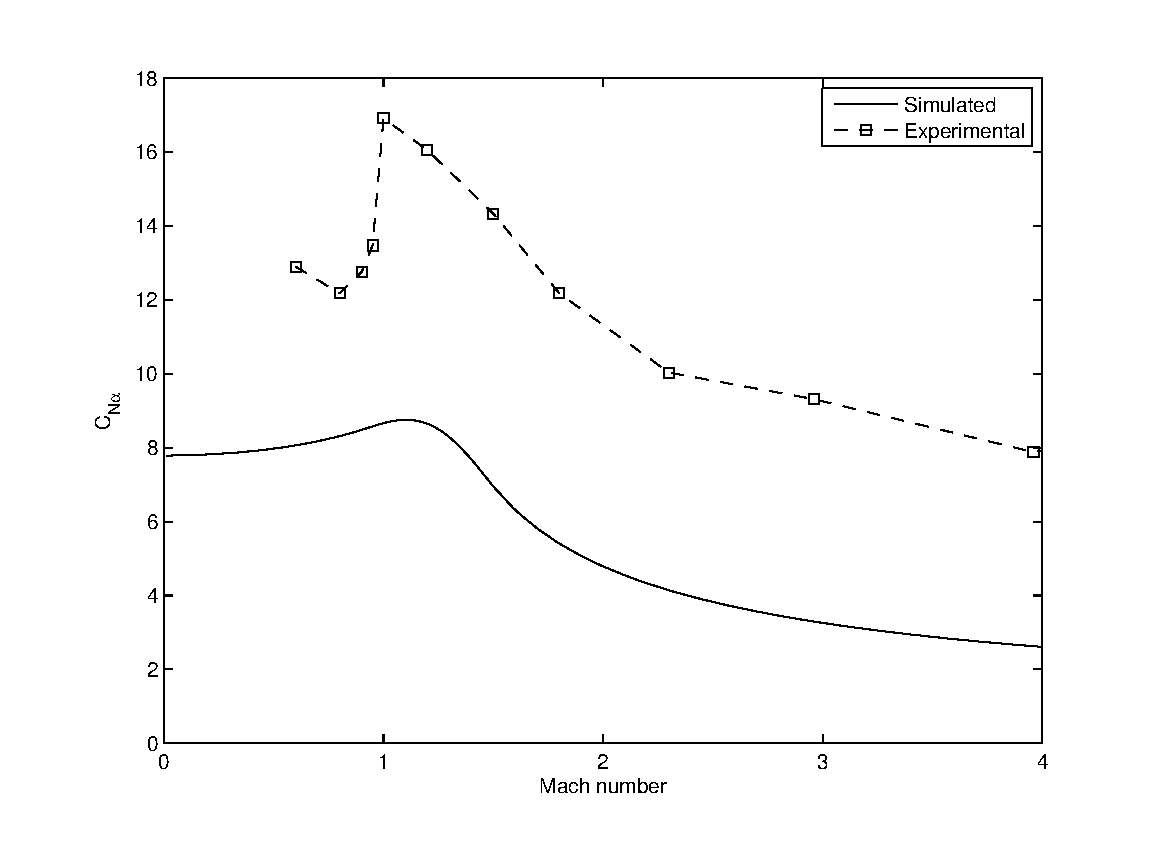
\epsfig{file=figures/experimental/cna-vs-mach,width=12cm} \\
(b)
\caption{Experimental and simulated center of pressure location (a)
  and normal force coefficient derivative (b) as a function of Mach
  number.}
\label{fig-experimental-CP-CNa}
\end{figure}

The CP location as a function of Mach number and the normal force
coefficient derivative \CNa\ are presented in
Figure~\ref{fig-experimental-CP-CNa}.  The 3\% error margins in the
transonic region were added due to difficulty in estimating the normal
force and pitch moment coefficient derivatives from the printed
graphs; in the supersonic region the CP location was provided
directly.  At subsonic speeds the CP location matches the experimental
results to within a few percent.  At higher supersonic speeds the
estimate is too pessimistic, and due to the interpolation this is
visible also in the transonic region.  However, the CP location is
quite reasonable up to about Mach~1.5.

The simulated normal force coefficient derivative is notably lower
than the experimental values.  The reason for this is unknown, since
in his thesis Barrowman obtained results accurate to about 6\%.  The
effect of the lower normal force coefficient on a flight simulation is
that the rocket corrects its orientation slightly slower than in
reality.  The effect on the flight altitude is considered to be small
for typical stable rockets.

